\section{Timeline}

Various Data Release Processing campaigns are required during Commissioning and in the runup to Operations, as follows:

\begin{description}

\item [DP0.2 (July 2021—September 2022)] -- a DRP experiment to reprocess data from DESC DC2 using topical LSST Pipeline software. This DRP experiment only involves a single data facility (the Interim Data Facility on the Google Science Cloud), but is a vital source of information for the three-site DRP capability, as it involves all of the fundamental elements of DRP.

\item [DP0.3 (timing to be confirmed)] -- a re-run of the DRP workflow used to create DP0.2, though running across the three Data Facilities rather than on the IDF. It will be worthwhile to compare the properties of the DP0.2 and DP0.3 campaigns, considering efficiency, resilience, and effectiveness, for example.

  ComCam is expected to be installed onto the Telescope Mount Assembly in February 2022, with the possibility the camera producing {\em on-sky images} before the end of 2022. Further, ComCam will produce a significant amount of calibration data, which can also be used for testing DRP.

  We should be able to process ComCam images at the US DF by June 2022 and it is also desirable to process BOT data.  
  
\item [DP1 (April 2022—March 2023)] -- data from the Commissioning Camera (ComCam), installed at the Observatory, will be processed twice: first, at NCSA (Construction DF); and, then, across the three Data Facilities.

  At the time of writing, {\em Engineering First Light} is expected to be in January 2023.

\item [DP2 (October 2022—December 2023)] -- Commissioning Data from the full LSST Camera, installed at the Observatory, will be processed across the three Data Facilities, aiming to mimic the conditions and timeline of a production DRP campaign as closely as possible.

\item [DR1 (July--December 2023)] Rubin Observatory operations are expected to begin in January 2024, with the raw images that will constitute the first, in-production, Data Release (DR1) being ready to process in July 2024.

\end{description}

\begin{itemize}

\item ComCam will go on the TMA next month

  \begin{itemize}

  \item We will have images, potentially on Sky images, before year end.

  \item We will have loads of calibration data

  \end{itemize}
  
\item We should be able to process ComCam images at SLAC in June.

  \begin{itemize}

  \item Would be nice to process all the BOT data

  \end{itemize}

\item Officially engineering first light is Jan 2023 (likely a little later)

  \begin{itemize}

  \item Then we need OGA racks etc.

  \item We will still be getting lots of engineering data from the real camera !

  \end{itemize}

\end{itemize}

The USDF timeline is in \citeds{RTN-021} the high level milestone chart is duplicated in \figref{fig:usdfplan} here.

\begin{figure}
\begin{centering}
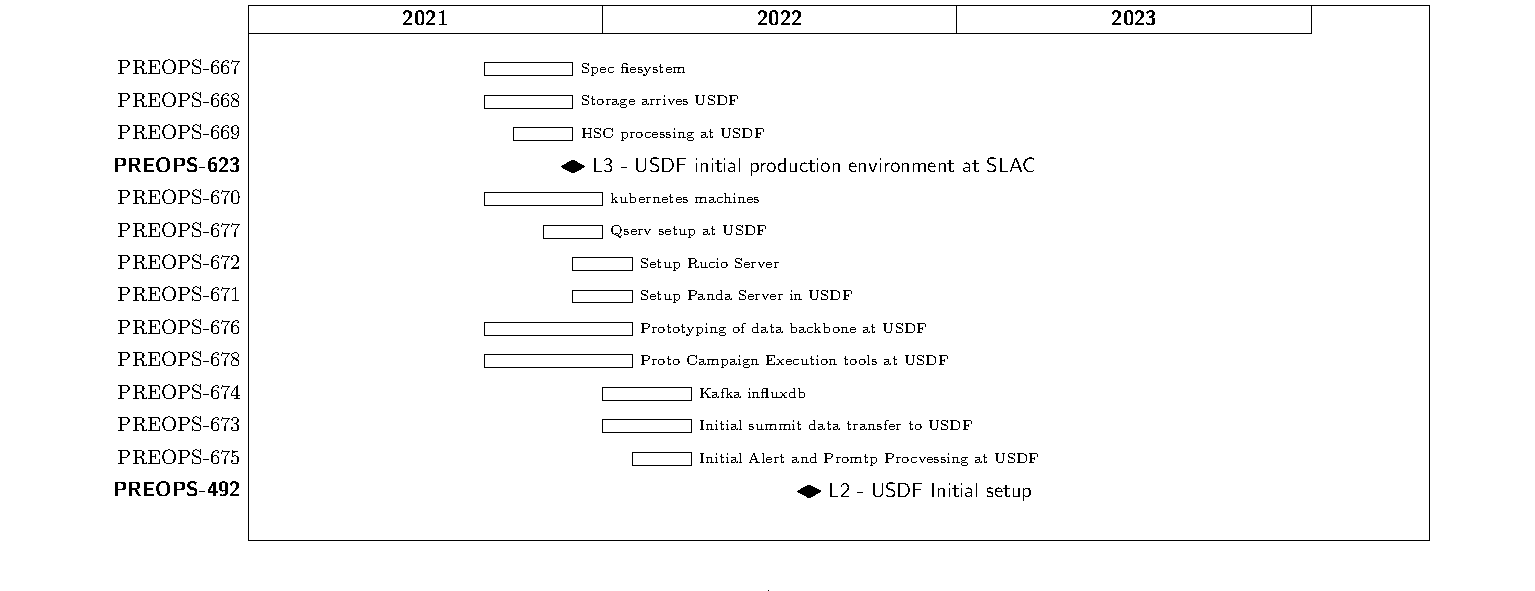
\includegraphics[width=0.9\textwidth]{USDFplan}
	\caption{USDF buildup plan from \citeds{RTN-021}\label{fig:usdfplan}}
\end{centering}
\end{figure}

The big question right now is {\em When can we start multi site testing with PanDA/Rucio ..
IDF, SLAC, FRdF all run PanDA \ldots}.

We need to build up tests for distributed processing RUCIO PanDA, which has started!


We need to make Jira Epics and capture decisions in technotes.

We need to agree interfaces between all the moving parts for the DFs to work with.
As always KISS!\footnote{Yes it is in the glossary.}


